%%%%%%%%%%%%%%%%%%%%%%%%%%%%%%%%%%%%%%%%%%%%%%%%
\section{Summary}


%%%%%%%%%%%%%%%%%%%%%%%%%%%%%%%%%%%%%%%%%%%%%%%%%%%
\begin{frame}

\frametitle{GitHub repository}

\dirtree{%
.1 .
.2 \myfolder{green}{data}\DTcomment{Data files}.
.3 \myfolder{green}{calgary}\DTcomment{Part of the Calgary corpus}.
.3 \myfolder{green}{canterbury}\DTcomment{Part of the Canterbury corpus}.
.2 \myfolder{red}{slides}\DTcomment{\LaTeX source of these slides}.
.2 src\DTcomment{All of the examples}.
.3 \myfolder{blue}{tools}\DTcomment{Perl and R scripts used}.
.3 \myfolder{blue}{v1}\DTcomment{Makefile example}.
.3 \myfolder{blue}{v2}\DTcomment{Single rule}.
.3 \myfolder{blue}{v3}\DTcomment{Two rules}.
.3 \myfolder{blue}{v4}\DTcomment{Generalisation}.
.3 \myfolder{blue}{v5}\DTcomment{Python in a run directive}.
.3 \myfolder{blue}{v6}\DTcomment{Final, largest example}.
}

The PDF of the slides are at the top directory.

\end{frame}


%%%%%%%%%%%%%%%%%%%%%%%%%%%%%%%%%%%%%%%%%%%%%%%%%%%
\begin{frame}

\frametitle{Snakemake $=$ Python}

{\red{$\rightarrow$}} Not really...
\vs

Since the developers made Snakemake with Python, there are many opportunities to leverage Python.
\begin{itemize}
  \item A Python function to return a list of inputs paths.
  \item A {\texttt{run}} directive (or {\texttt{script}} directive) that accepts Python code.
\end{itemize}
\vs

But, you can write a Snakemake workflow without calling any Python code.

\end{frame}


%%%%%%%%%%%%%%%%%%%%%%%%%%%%%%%%%%%%%%%%%%%%%%%%%%%
\begin{frame}

\frametitle{Snakemake $=$ ``reproducibility''}

{\red{$\rightarrow$}} Unfortunately, no...
\vs

We are all looking for that ``magical'' method.  If this method is used, then reproducibility of our analysis is ``guaranteed''.
\vs

Snakemake {\red{is}} a step in the right direction.  But using it alone does not guarantee reproducibility.

\end{frame}


%%%%%%%%%%%%%%%%%%%%%%%%%%%%%%%%%%%%%%%%%%%%%%%%%%%
\begin{frame}

\frametitle{Analogy}

Snakemake defines a workflow, which is analogous to a recipe for baking.  If you follow it, you will get the same cake every time.
\vs

But suppose the recipe asks for whole milk and, for whatever reason, whole milk is no longer available anywhere.  You will need to substitute it with skim milk or oat milk (for example).  Even if you still use the same quantity as the recipe, the end result will not be the same.
\vs

Something outside of the recipe (and beyond your control) has made reproducibility not possible.

\end{frame}


%%%%%%%%%%%%%%%%%%%%%%%%%%%%%%%%%%%%%%%%%%%%%%%%%%%
\begin{frame}[fragile]

\frametitle{More concrete example}

This appears in one of the Perl scripts today:

\begin{tiny}
\begin{lstlisting}[frame=single,language=perl]
use AppConfig;
use AppConfig::Getopt;
\end{lstlisting}
\end{tiny}

It allows a Perl script to process arguments on the command-line.  On my system, version 1.71-2.3build1 of AppConfig was used.  Years later, this version might be too old and version 2.00 (for example) might be needed.
\vs

There are ways to {\magenta{lock}} (or pin) libraries down to an exact version to address this problem.  But if the system administrator tells you that version 1.71-2.3build1 has a serious security flaw and ``you must upgrade'' or ``you will not be allowed to run it'', then you have no choice. 

\end{frame}


%%%%%%%%%%%%%%%%%%%%%%%%%%%%%%%%%%%%%%%%%%%%%%%%%%%
\begin{frame}

\frametitle{Support of Jupyter notebooks?}

{\red{$\rightarrow$}} Unfortunately, no...
\vs

I am not an expert on Jupyter notebooks, but they seem to be very good at {\green{interactive}} analysis of data.  Similar to RStudio.
\vs

With Snakemake, you need to write scripts (i.e., Python, R, etc.) that are not interactive.  Parameters can be supplied to affect how the program is run.

\end{frame}


%%%%%%%%%%%%%%%%%%%%%%%%%%%%%%%%%%%%%%%%%%%%%%%%%%%
\begin{frame}

\frametitle{Support for SLURM/CSF3?}

{\red{$\rightarrow$}} Yes!
\vs

Over 5 years ago, I created Snakemake scripts that would send $x$ (which you specify) jobs to SLURM.  As your my jobs completed, new ones are added so that there are always around $x$ jobs running / queued.
\vs

Looking at the documentation, the method to do this appears to have changed.  Now, it might called {\href{https://snakemake.readthedocs.io/en/v9.18.1/executing/executors.html}{{\red{executors}}}}.
\vs

The problem for CSF3 is that you need your Snakemake script to be {\magenta{continuously}} running on the login node.

\end{frame}


%%%%%%%%%%%%%%%%%%%%%%%%%%%%%%%%%%%%%%%%%%%%%%%%%%%
\begin{frame}

\frametitle{Support for SLURM/CSF3}

E-mail from September 2026:
\begin{figure}
  \centering
  {\fbox{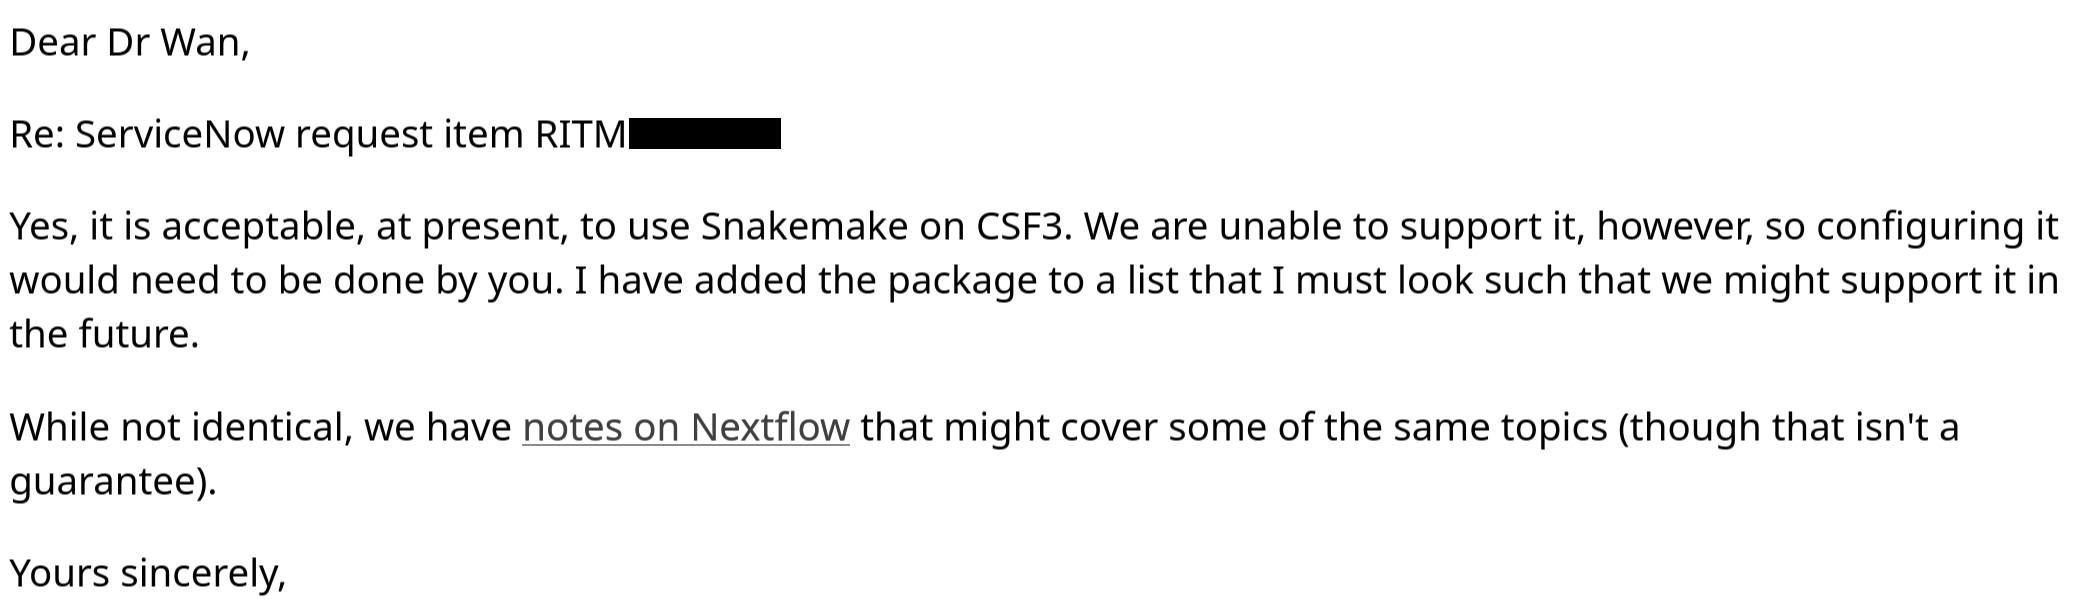
\includegraphics[width=\linewidth]{summary/csf3}}}
\end{figure}

Link in message:  \href{https://ri.itservices.manchester.ac.uk/csf3/software/applications/nextflow/}{https://ri.itservices.manchester.ac.uk/csf3/software/applications/nextflow/}

\end{frame}


%%%%%%%%%%%%%%%%%%%%%%%%%%%%%%%%%%%%%%%%%%%%%%%%%%%
\begin{frame}

\frametitle{Summary}

\begin{itemize}
  \item If you're using {\texttt{bash}} scripts or copy-and-pasting commands in from a lab notebook for a workflow consisting of many steps, you should consider some workflow-based system.
  \item Snakemake is one of many options.
  \item Of course, if you only run only a few commands, then Snakemake might be more than what you need!
\end{itemize}

\end{frame}


